\chapter{Perancangan}
\label{chap:perancangan}

Pada bab ini akan dijelaskan perancangan mengenai simulator yang akan dibangun untuk pertumbuhan wirausaha.

\section{Perancangan Kelas}
\label{sec:perancangankelas}

Dalam membuat simulator diperlukan sebuah GUI atau Interface untuk bisa menggambarkan kinerja suatu sistem. Berdasarkan hasil pengembangan diagram kelas pada bab analisis \ref{fig:CD1}, dibuatlah diagram kelas rinci untuk memenuhi kebutuhan dalam membangun simulator. Deskripsi kelas beserta fungsi dari diagram kelas akan dijelaskan pada subbab selanjutnya.

\begin{figure} [H]
	\centering  
	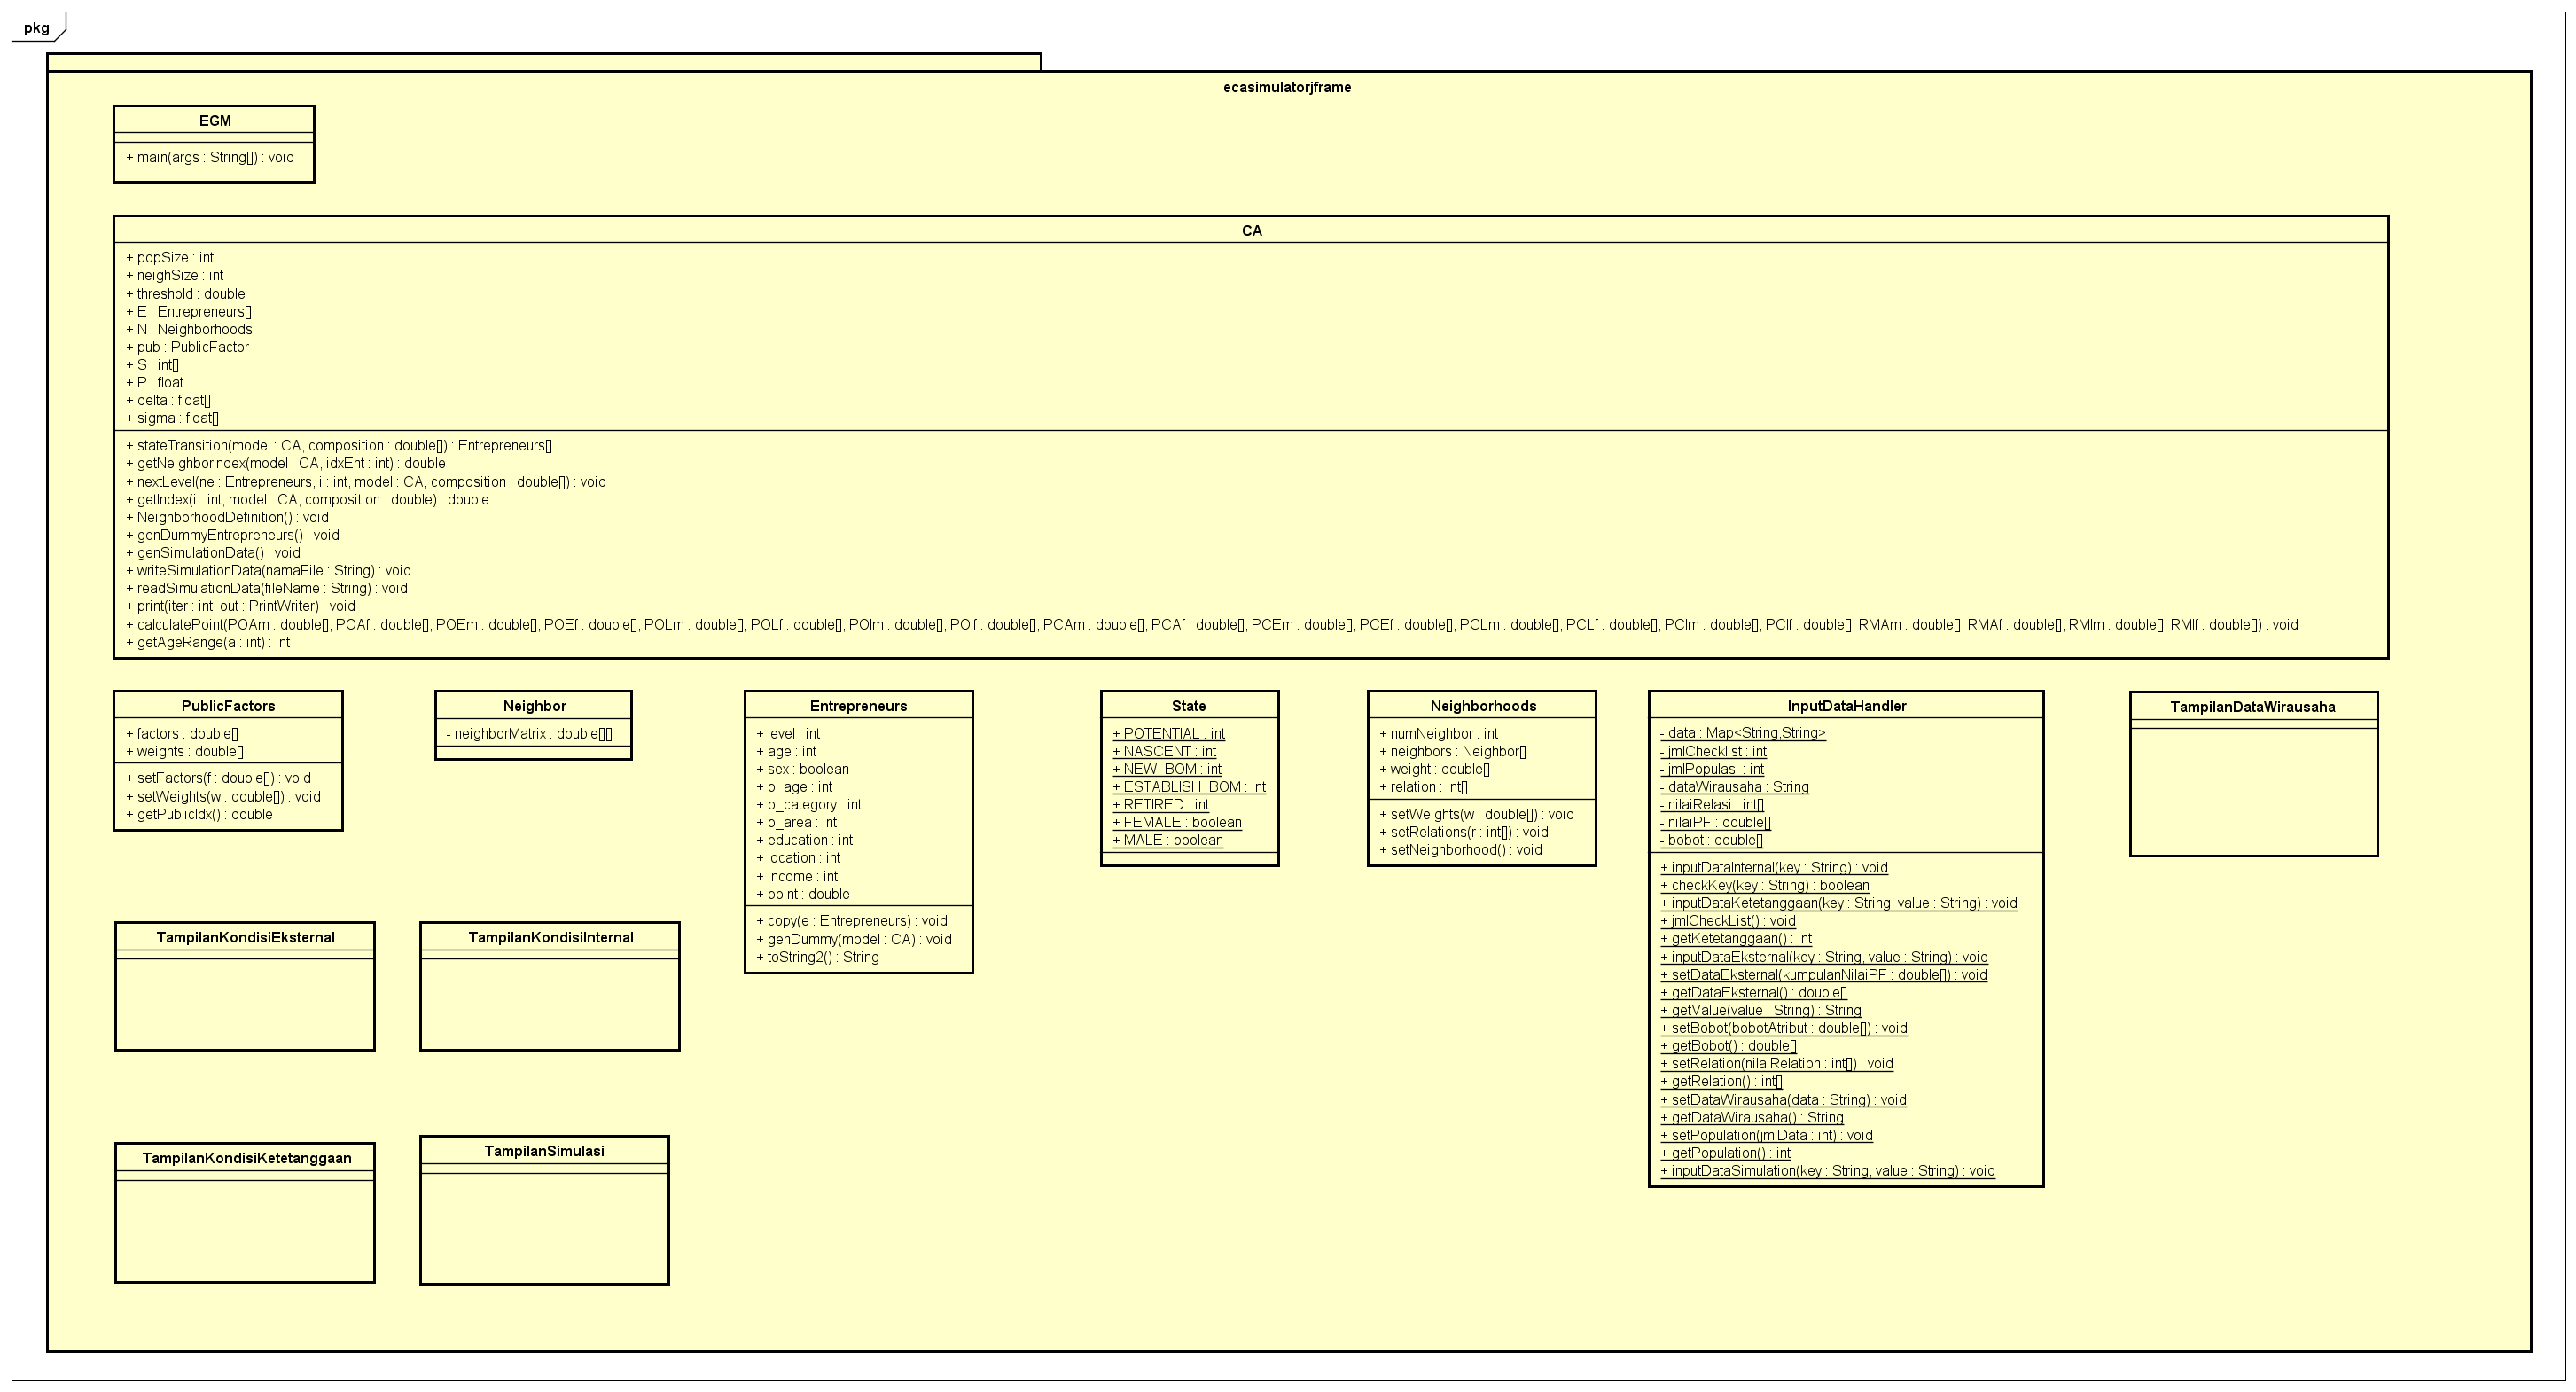
\includegraphics[width=18cm, height=12cm]{ClassDiagram2} 
	\label{fig:classdiagram2} 
\end{figure}

\subsection{Kelas TampilanKondisiInternal}
Kelas ini merupakan kelas untuk menampilkan seluruh atribut umum dari seorang wirausaha yang dapat dipilih menggunakan \textit{checkbox}, atribut yang dipilih nantinya akan mempengaruhi ketetanggaan antara wirausaha yang satu dengan wirausaha lainnya. Setelah itu, \textit{user} diminta mengisi bobot untuk masing-masing atribut yang sudah dichecklist melalui \textit{textfield}.

\subsection{Kelas TampilanKondisiKetetanggaan}
Kelas ini merupakan kelas untuk menampilkan atribut yang sudah dipilih dari kelas TampilanKondisiInternal. \textit{User} dapat memilih atribut mana saja yang akan 
\subsection{Kelas InputDataHandler}
Kelas ini merupakan kelas untuk mengambil dan menyimpan data masukan dari \textit{user}. 